The next step in designing a PCB is creating the layout with the program Pcbnew included in the KiCad EDA suite.  The following work order is used when designing the layout of the PCB:

\paragraph{Setup PCB layers}

The top and bottom layers are used for signal routing; the inner layer near the top side is used for analog and digital ground planes; and the inner layer near the bottom side is used for analog and digital power planes.

\paragraph{Setup design constraints}
	
Design rules in Pcbnew are set to comply with the manufacturer design constraints in~\cite{AdvCir66} and~\cite{AdvCirTol}. Default trace widths are set to $0.008\unit{in}$ with $0.016\unit{in}$ width for power traces on the signal layers, and to save board area, the via drill size is set to the minimum $0.015\unit{in}$~\cite{AdvCir66}.  Blind and buried vias are not allowed~\cite{AdvCir66}.
	
\paragraph{Import netlist}

Pcbnew imports the netlist file created by Eeschema and CvPcb and places all of the component footprints in the layout window with vector lines representing connections between pins, creating the ``rats nest''~\cite{PcbnewRefMan}.

\paragraph{Draw PCB outline}

The board outline is drawn as a $4.75\unit{in}$ square, which matches the dimensions of the RTSC board.  

\paragraph{Place connectors}

Placement of the Hirose FX2 connector is critical to ensure proper mating with the connector on the RTSC board, and the PCI-Express connectors are placed close to the recording electrode terminal block the keep the trace length short.
	
\paragraph{Place remaining components}

The remaining components are placed on the top layer with some exceptions for resistors and capacitors.  Analog and digital components are placed while being mindful of the need to keep them above the analog and digital ground planes, respectively, without overlap.  Decoupling and Bypass capacitors are placed as close as possible to power pins and connectors, preferring to place the capacitors on the same side as the component.

\paragraph{Draw ground and power planes}

The power and ground planes are drawn on the inner layers in shapes that preserve analog and digital isolation and minimize trace length to the power and ground pins of components.  Figures~\ref{fig:PCBGND} and~\ref{fig:PCBPWR} show the ground and power planes, respectively, of the Electrophysiology Interface board.  Care must be taken to ensure that the copper planes maintain the minimum clearance around component and via holes ($0.010\unit{in}$ for inner layers) and the PCB edge ($0.015\unit{in}$ for inner layers) while also ensuring that the plane is continuous~\cite{AdvCirTol}.  Figure~\ref{fig:vitalclear} shows two locations on the power and ground layers where the plane clearance is vital to maintaining continuous planes.

Figure~\ref{fig:vitalPWR} shows where the +VA plane has a through-hole connector occupying the full height of the plane.  If the clearance between the plane and the hole features is too large, the plane will not be filled between the holes, disconnecting parts of the plane.  Likewise, in Figure~\ref{fig:vitalGND}, many pins on the two rows closest to the board edge need to connect to the DGND net; a large plane clearance will cut off the pins from the ground plane.

\begin{figure}[h]
	\begin{singlespace}
	\centering	
		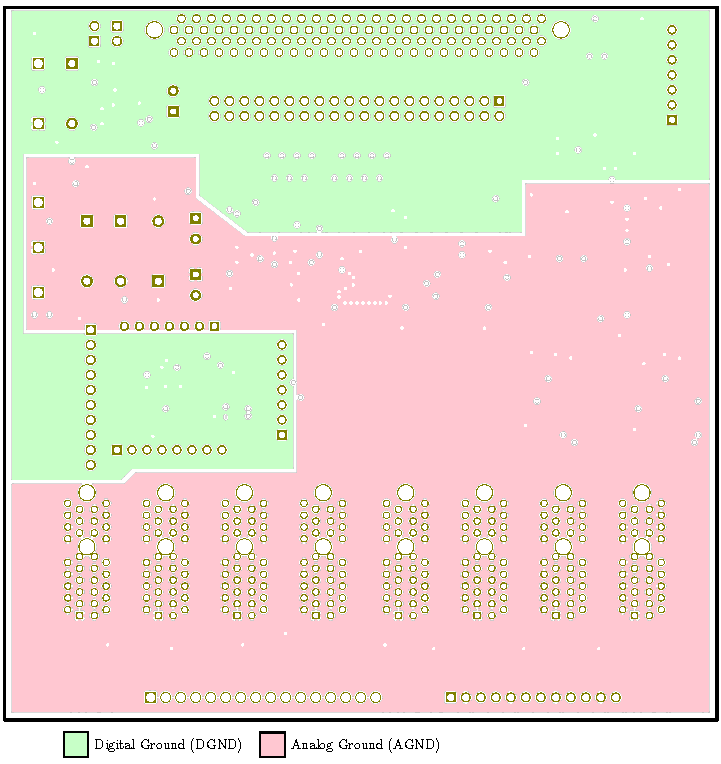
\includegraphics{./figures/PCBCopperGND} 
	\caption{PCB ground plane layer\label{fig:PCBGND}}
	\end{singlespace}
\end{figure}

\begin{figure}[h]
	\begin{singlespace}
	\centering 
		\includegraphics{./figures/PCBCopperPWR} 
	\caption{PCB power plane layer\label{fig:PCBPWR}}
	\end{singlespace}
\end{figure}

\begin{figure}[h]
	\centering 
	\begin{singlespace}
	\begin{subfigure}[b]{0.35\textwidth}
		\centering 
		\includegraphics[trim=1in 1.25in 3in 3.5in,clip,width=\textwidth]{./figures/PCBCopperPWR} %[trim=left bottom right top]
	\caption{Power plane\label{fig:vitalPWR}}
	\end{subfigure}
	~
	\begin{subfigure}[b]{0.35\textwidth}
		\centering 
		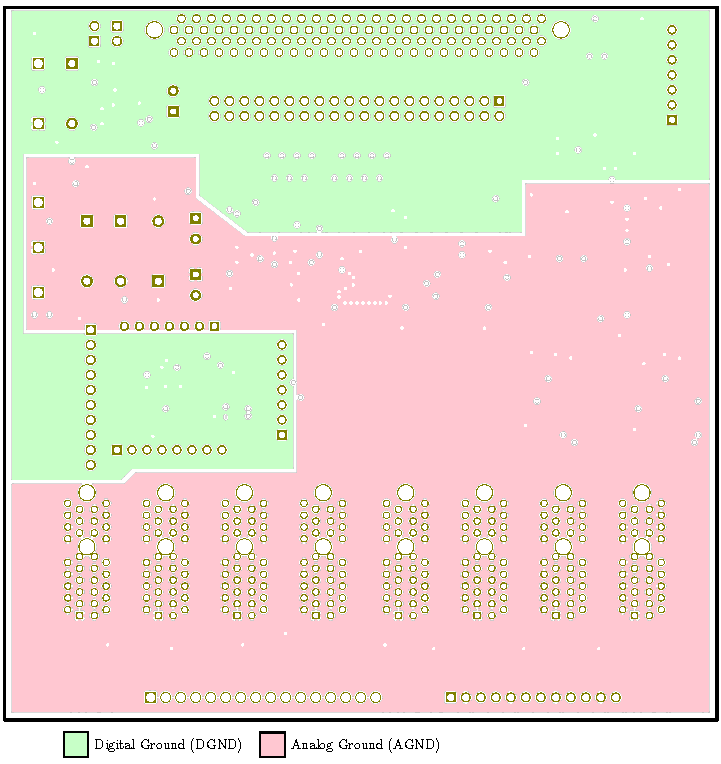
\includegraphics[trim=0.9in 4.7in 3.25in 0in,clip,width=\textwidth]{./figures/PCBCopperGND} %[trim=left bottom right top]
	\caption{Ground plane\label{fig:vitalGND}}
	\end{subfigure}
	\caption{Close clearances on power and ground planes\label{fig:vitalclear}}
	\end{singlespace}
\end{figure}

\paragraph{Route critical signal traces}

The signals most susceptible to signal integrity issues should be routed first.  These signals include the high-frequency digital signals between the FPGA, ADC, and DAC and the noise susceptible signal from the recording electrodes.  The traces should be routed with minimum length, through as few vias as possible, and on the layer adjacent to the ground plane~\cite{Montrose1999}.

\paragraph{Route remaining traces}

After the components are placed, ground planes drawn, and susceptible traces routed, the remaining signal traces may be routed.  To avoid disfigurement of the trace during the etching process, narrow traces are routed so that they never form a right angle: they first turn $45^\circ$, then they extend at least a short distance, and finally they can make another $45^\circ$ turn~\cite{ExpresssPCBTips}.  Figure~\ref{fig:PCBTopBot} shows the traces and pads on the top and bottom layers of the PCB.

\begin{figure}[htb]
	\begin{singlespace}
	\centering 
		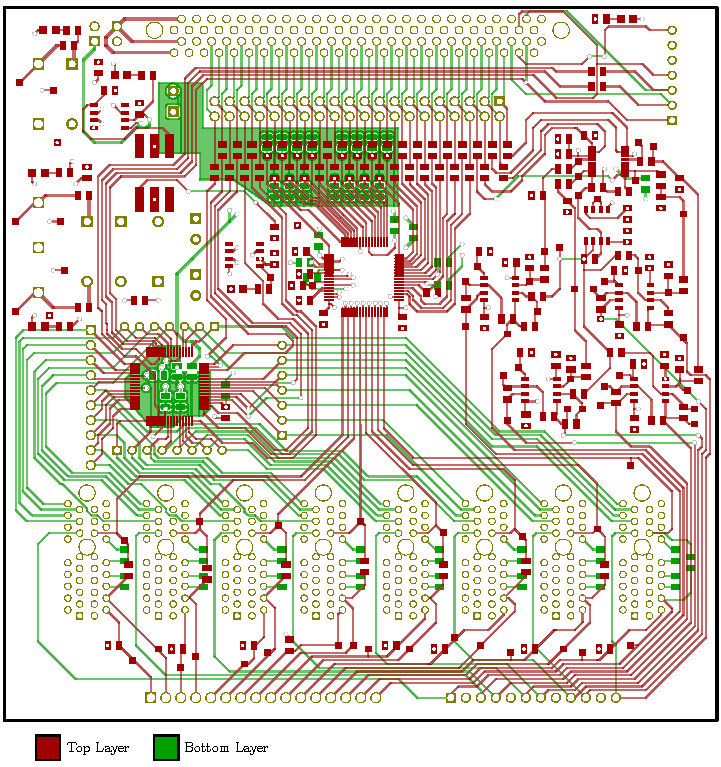
\includegraphics{./figures/PCBCopperTopBot} 
	\caption{PCB top and bottom signal layers\label{fig:PCBTopBot}}
	\end{singlespace}
\end{figure}
	
\paragraph{Place test points}

After the traces are routed is the best time to place the test points on the board.  The placement of the test point pads is not critical for the Electrophysiology Interface board, but the size of the pad can interfere with trace routing; thus, the test points can be located last.  The test point pads should be placed so as to be accessible after the components are populated.
	
\paragraph{Iterate this procedure as needed based on signal routing}

To adapt to the challenges encountered during signal routing, it is necessary to adjust ground and power planes, move components, edit component footprints, and change signal connections on the schematic.  For instance, the CPLD connections to the Preamp connectors are entirely based on the routing needs of the board layout.

\paragraph{Move labels on the silkscreen layer}

Finally, after all the signals are successfully routed, the reference designators for the individual components should be moved so that the labels are visible after the parts are populated on the board, allowing physical parts to be matched to the components in the schematic.  Labels should not be located under parts or on top of exposed copper pads.



